\documentclass[12pt, letterpaper]{article}

\usepackage{graphicx} % Required for inserting images
\usepackage[margin=1in]{geometry} % Sets 1-inch margins
\usepackage{titlesec}
\usepackage{setspace}
\usepackage{mathptmx}
\usepackage{titlesec}
\usepackage{amsmath}
\usepackage{amssymb}
\usepackage{fancyhdr}
\usepackage{lastpage}
\usepackage{tocloft}
\usepackage{float}
\usepackage{subcaption}
\usepackage{hyperref}
\usepackage{bm}
\usepackage{comment}

\setlength{\parindent}{0pt}  % Disable paragraph indentation
\setlength{\parskip}{1em}   % Add space between paragraphs
\titlespacing*{\section}{0pt}{0.5em}{0em} % Section: 1em before, 0.5em after
\titlespacing*{\subsection}{0pt}{0em}{0.4em} % Subsection: 0.8em before, 0.4em after
\onehalfspacing
\titleformat{\section}{\normalfont\large\bfseries}{\thesection}{1em}{}
\titleformat{\subsection}{\normalfont\normalsize\bfseries}{\thesubsection}{1em}{}
\titleformat{\subsubsection}{\normalfont\small\bfseries}{\thesubsubsection}{1em}{}

\pagestyle{fancy} % Enable custom headers and footers
\renewcommand{\headrulewidth}{0pt}
\fancyhead[L]{Stabilization and Bifurcation of the Inverted Pendulum}   % Left side of the header
\fancyhead[R]{Belinsky, Finkelstein}  % Right side of the header

\fancyfoot[L]{M638-01 Spring, 2025}   % Left side of the footer
\fancyfoot[C]{} % Center of the footer (page number)
\fancyfoot[R]{\thepage\ of \pageref{LastPage}}  % Right side of the footer


\title{Stabilization and Bifurcation of the Inverted Pendulum}  % Set the title
\author{P. Belinsky ~E. Finkelstein  \\        % Set the author(s)
\small San Diego State University}
\date{\today}



\begin{document}
\raggedright
\vspace{2cm}
\maketitle
\vspace{2cm}
\begin{abstract}
We explore the dynamical stabilization of the inverted pendulum under vertical periodic forcing and the bifurcation behavior of the full nonlinear system. Beginning with a rigorous time-averaging analysis, we examine the conditions under which the inverted position becomes stable and subsequently map out stable regions in the undamped Mathieu parameter space with Floquet multipliers. We then investigate the full nonlinear dynamics, including the appearance of limit cycles and bifurcations, through Poincaré maps and Floquet theory. We give special attention to the \emph{transition mechanisms}—such as pitchfork and period-doubling bifurcations—that lead to complex dynamical behavior. Our findings extend prior work with a more insightful time-averaging analysis and a detailed numerical examination of bifurcations beyond initial instability events.
\end{abstract}

\newpage
\begingroup
\setlength{\cftbeforesecskip}{0pt}  % Remove space before section entries
\setlength{\cftsecindent}{0pt}      % Remove indentation of section titles
\renewcommand{\baselinestretch}{1}  % Set single spacing for TOC
\tableofcontents
\thispagestyle{fancy}  % Apply the custom header/footer to the TOC page
\endgroup
\listoffigures
\newpage  % Start content on a new page

\section{Introduction}
The pendulum is a canonical model for studying the mathematical representation and stability of physical, continuous-time systems of the form \cite{strogatz2018nonlinear}:
\begin{align}
    \dot{x}_1 &= f_1\left(x_1, \ldots, x_n\right) \nonumber \\ 
    &\vdots \nonumber \\ 
    \dot{x}_n &= f_n\left(x_1, \ldots, x_n\right) \label{eq:general_system_framework},
\end{align}
where $x_i$ are the state variables and the $\dot{x}_{i=1,\ldots,n} \equiv d{x}_{i=1,\ldots,n}/dt$ terms denote how the state variables change in time. 
\par As recounted in \cite{dolan2017inverted}, the pendulum system has been physically studied ever since Galileo Galilei (see, e.g. \cite{drake2003galileo} for a thorough biography), who, famously, as a blind man at 77, theorised with his son Vincenzo Gamba the pendulum clock in 1641 that was later built to completion and patented by Christiaan Huygens on June 16, 1657, who, quite relevantly for this paper, appears to be credited with deriving the formula for the natural period of the mathematical pendulum \cite{aps_huygens_2017}:
\begin{equation}
    T = 2\pi \omega_0 = 2\pi\sqrt{\dfrac{g}{l}} \label{eq:natural_period_math_pendulum}
\end{equation}

\par A particularly intriguing behavior exhibited by the pendulum system is the dynamic stabilization of the inverted position through vertical oscillations of the pivot point. The first observation of this phenomenon was by Andrew Stephenson, who in 1908 reported this stabilization to be a result of fast, vertical (parallel to the force of gravity), periodic oscillations of the pivot point \cite{Stephenson1908XXOI}. It wasn't until 1951; however, that Pyotr Leonidovich Kapitsa derived the \emph{physical mechanism} that causes the upright position to become stable \cite{kapitsa1951jetp}. Before his work, the stability of the pendulum could only be probed mathematically with approximations such as truncated Hill determinants of the corresponding Mathieu equation \cite{kapitsa1951jetp}.

\par Since 1951, there has been extensive research into the conditions needed to stabilize the inverted position. Methods such as time-averaging techniques, linearization, and connections to the Mathieu equation are sufficient to fully understand the stability. The parameter space for stabilization is visualized with a diagram related to the Mathieu equation known as the Ince-Strutt diagram. Many papers, such as Butikov's 2017 paper \cite{Butikov2017KapitzaS}, offer insight into the physical intuition while still providing the mathematical rigor behind these results, making this a very accessible problem. However, understanding the application of the time-averaging method remains difficult. 

While it is most standard to analyze the stability of the inverted position, recent papers \cite{kim1998hu} dive into the full nonlinear, damped dynamics of the system. Notably, it has been found that there is a resurrection of stability of the inverted position as the amplitude of the oscillation increases. These studies also reveal the existence of bifurcations into limit cycles using a Poincare section and Floquet theory. These bifurcations come in complex sequences of period doubling to pitchfork bifurcations. Although these sequences are rich in dynamics, the existing literature only presents the initial bifurcation events. The bifurcation diagram beyond the first instability along with the respective phase portrait of these orbits remains underexplored. 

In this paper we aim to revisit the foundational knowledge of the pendulum and branch into an analysis of the bifurcation of the full nonlinear system. The paper is structured as follows: In section \ref{sec:dny_systems_eq_points_stab}, we'll introduce the canonical Kapitza pendulum dynamical system, analyze its components and stability through a rigorous, time-averaging physics study that extends Butikov's paper's analysis \cite{Butikov2017KapitzaS}, and then build on this study with a more mathematical but general analysis centered around probing the linearized system's Mathieu stability with Floquet theory. In section \ref{sec:nonlinear_dynamics}, we extend the linear stability analysis by reviewing Kim and Hu's studies examining the full damped, nonlinear system. We uncover the existence of limit cycles and characterize bifurcation phenomena—such as period doubling and pitchfork bifurcations—using Poincaré maps and Floquet theory. Finally, we conclude by summarizing our findings and discussing potential directions for further study.

%we will fill this in when we're done writing the paper so that we're accurate. 
%also I want to add a couple more references, I liked the brief historical background so i'll probably work that in somewhere somehow -> done ✅

% Can delete the below afaik
% \begin{comment}
% Chaos theory emerged from the observation of systems which dramatically change trajectory due to minuscule perturbations. The \emph{attribute} of chaos in the overarching field of \emph{dynamics}, while ``loosely'' defined, can only arise in continuous-time dynamical systems of $n \geq 3$ equations of the following form \cite{strogatz2018nonlinear}:
% \begin{align}
%     \dot{x}_1 &= f_1\left(x_1, \ldots, x_n\right) \nonumber \\ 
%     &\vdots \nonumber \\ 
%     \dot{x}_n &= f_n\left(x_1, \ldots, x_n\right) \label{eq:general_system_framework},
% \end{align}
% where $x_i$ are the state variables and the $\dot{x}_{i=1,\ldots,n} \rightarrow d{x}_{i=1,\ldots,n}/dt$ terms denote how the state variables change wrt. time. 
% \par In our project, we study a mathematical model for a type of \emph{pendulum}; a structure consisting of a rod-like extension connecting a mass of some sort to a pivot point about which the mass rotates \cite{merriamwebster_pendulum}. Specifically, we look at the case where the pivot point oscillates sinusoidally up and down, parallel to the force of gravity, a pendulum system known as the \emph{Kapitza pendulum} \cite{kapitsa1951jetp}, and shall investigate the mechanism(s) by which the inverted position can be stabilized and the parameters for which the system can bifurcate and undergo limit cycles and chaos.

% \section{Brief Historical Background on the Pendulum}
% % As recounted in \cite{dolan2017inverted}, the pendulum system has been physically studied ever since Galileo Galilei (see e.g. \cite{drake2003galileo} for a thorough biography), who, famously, as a blind man at 77, theorised with his son Vincenzo Gamba the pendulum clock in 1641 that was later built to completion and patented by Christiaan Huygens on June 16, 1657, who, quite relevantly for this paper, appears to be credited with deriving the formula for the natural period of the mathematical pendulum \cite{aps_huygens_2017}:
% % \begin{equation}
% %     T = 2\pi \omega_0 = 2\pi\sqrt{\dfrac{g}{l}} \label{eq:natural_period_math_pendulum}
% % \end{equation}
% \par The first documented observation/description of the stabilization of a pendulum in its upright equilibrium position was by Andrew Stephenson in 1908, who documented this stabilization as a result of fast, vertical (parallel to the force of gravity), periodic oscillations of the pivot point \cite{Stephenson1908XXOI}. 
% \par It wasn't until 1951 that Pyotr Leonidovich Kapitsa derived the \emph{physical mechanism} that causes the upright position to become stable \cite{kapitsa1951jetp}. Before this work, the stability of the pendulum could only be probed mathematically with approximations such as truncated Hill determinants of the corresponding Mathieu equation \cite{kapitsa1951jetp}.
% \end{comment}

\section{Dynamical System, Equilibrium Points, and Stability}\label{sec:dny_systems_eq_points_stab}
The dynamical system for the Kapitza pendulum \cite{kapitsa1951jetp}, typically derived using Newton's second law or the Euler-Lagrange equations\footnote{the latter approach included in section \ref{sec:el_derivation_butikov_eom} for completeness} is given in \cite{Butikov2017KapitzaS} by the equation: 
\begin{equation}
    \ddot{\phi} + 2\gamma\dot{\phi} + \left(\dfrac{g}{l} - \dfrac{a}{l}\omega^2 \cos(\omega t)\right)\sin(\phi) = 0            
    \label{eq:Kapitza_pendulum_system},
\end{equation}
where $\phi(t)$ is the time-dependent angular deflection of the pendulum from the vertical axis (note $\phi=0$ radians denotes the bottom position and $\pi$ radians the inverted position), $g$ is the acceleration due to gravity (around \href{https://physics.nist.gov/cgi-bin/cuu/Value?gn}{$9.81 \text{ m/s}^2$} on Earth), and $l$ is the length of the massless, taught rod connecting the pivot point to the opposite point of mass $M$. Unique to the Kapitza pendulum, the pivot point undergoes a parallel-to-gravity sinusoidal oscillation of the form 
\begin{equation}
    z(t) = a\cos(\omega t) \label{eq:pivot_point_osc_function},
\end{equation}
 where $a$ is the oscillation amplitude and $f=\omega/2\pi$ the number of oscillations per second. Lastly, a damping term controlled by the parameter $\gamma$ is included in \ref{eq:Kapitza_pendulum_system} (from \cite{Butikov2017KapitzaS}) and is therein assumed to be proportional to the rate of change of $\phi$ wrt. time, i.e., $\dot{\phi}$. Equation \ref{eq:Kapitza_pendulum_system} can be written in the form of \ref{eq:general_system_framework}, namely: 
\begin{align}
      \bm{\Phi} = \begin{pmatrix} \dot{\phi}_1 \\ \dot{\phi}_2 \\ \dot{t} \end{pmatrix} = \begin{pmatrix} \phi_2 \\ -2\gamma\phi_2 - \left(\dfrac{g}{l} - \dfrac{a}{l}\omega^2 \cos(\omega t)\right)\sin(\phi_1) \\ 1 \end{pmatrix} \label{eq:Kapitza_pendulum_gen_framework_form},
\end{align}
where the change of variables applied to \ref{eq:Kapitza_pendulum_system} is $\phi_1 \equiv \phi$, $\dot{\phi} = \dot{\phi}_1 = \phi_2$, $\dot{\phi}_2 = \ddot{\phi}_1 = \ddot{\phi}$.
\par The non-autonomous system \ref{eq:Kapitza_pendulum_gen_framework_form} clearly has no fixed points (points were $\bm{\Phi} = 0$). Instead, the system may exhibit periodic orbits. In this section, in lieu of an anlytical solution, we'll apply and numerically validate different techniques for ascertaining regions in parameter space corresponding to \emph{stable} periodic orbits, i.e., orbits that nearby nearby trajectories converge to over time.
\subsection{Time-Averaging} \label{subsec:time_averaging}
Figure \ref{fig:butikov_2017_figure_2} shows an example reproduced from \cite{Butikov2017KapitzaS} of the system \ref{eq:Kapitza_pendulum_gen_framework_form} numerically integrated with an initial condition $\phi_1(0) = 200^\circ$, $\phi_2(0) = 0$. 

\begin{figure}
    \centering
    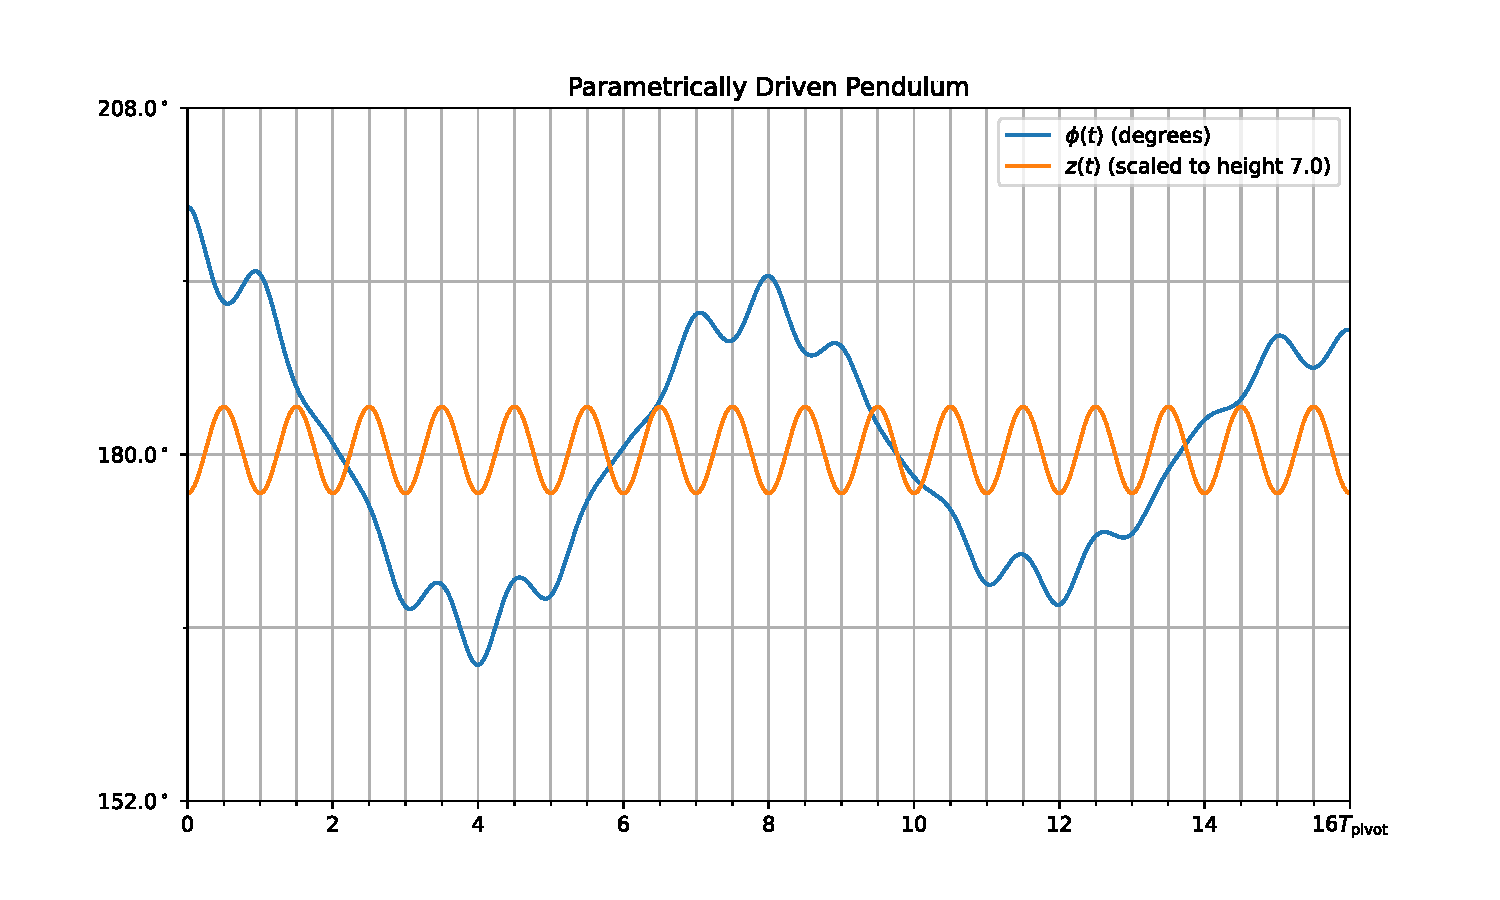
\includegraphics[width=0.5\linewidth]{ButikovKapitza2017Figure2.pdf}
    \caption{Numerical integration of \ref{eq:Kapitza_pendulum_gen_framework_form}, independently reproduced from Figure 2 of \cite{Butikov2017KapitzaS} which uses $a = 0.2l$, $\omega = 16 \omega_0$, $T = \dfrac{2\pi}{\omega} = \dfrac{\pi}{8\omega_0}$, $T_{\mathrm{Final}} = 16 T = \dfrac{2\pi}{\omega_0}$, $Q = 5 = \dfrac{\omega_0}{2\gamma} \Rightarrow \gamma = \dfrac{\omega_0}{10}$. The specific values chosen for this plot where $g = 9.81$ and $l = 100$; however, the results appear the same for any given values given the same ratios.}
    \label{fig:butikov_2017_figure_2}
\end{figure}

It is evident that, for this example, the pendulum bob undergoes roughly 2 periods of oscillation about the inverted position $\phi_1=180^{\circ}$ through 16 periods of the pivot point oscillation. Thus the ratio of the fast and slow frequencies is roughly:
\begin{equation}
    \text{Frequency Ratio} = \frac{\omega_{\text{pivot point}}}{\omega_{\text{pendulum bob}}} \approx \frac{16}{2} = 8
\end{equation}

It is readily apparent that there are two separate time-scales in this example, namely, a fast time scale (the driving frequency) and a slow time (the frequency of the pendulum bob's oscillations about $\phi = 180^\circ$). From this, Butikov proceeds to recount an approximate analytical stabilization criterion by splitting the deflection angle $\phi(t)$ into a superposition of two functions; $\theta(t)$ that varies slowly in time and $\delta(t)$ that varies quickly with frequency $\omega$, so that $\phi(t) = \theta(t) + \delta(T)$ becomes a sum of fast and slow parts. 
\par To illustrate the two-timing mechanism more readily, Figure \ref{fig:ButikovKapitzaFig3bTopMoreDetailedGravity} shows a schematic diagram of the Kapitza pendulum as described in \cite{Butikov2017KapitzaS}.
\begin{figure}
    \centering
    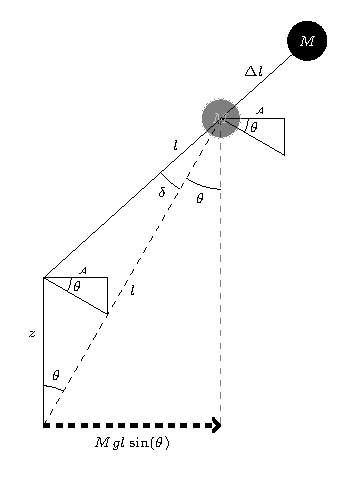
\includegraphics[width=0.8\linewidth]{ButikovKapitzaFig3bTopMoreDetailedGravity.pdf}
    \caption{Schematic diagram of the Kapitza pendulum, created for the purpose of more easily illustrating the derivation of $\left<V_{\mathrm{eff}}\right>$ Butikov recounts in \cite{Butikov2017KapitzaS}.}
    \label{fig:ButikovKapitzaFig3bTopMoreDetailedGravity}
\end{figure}
Here, $z(t)$ is the height of the pivot point displacement, the angle $\theta(t)$ is the angle of the pendulum rod wrt. the vertical, and $\delta(t)$ measures the angle corresponding to the height of the pivot point $z$. As we saw in the stabilized case of Figure \ref{fig:butikov_2017_figure_2}, $\delta(t)$ varies quickly compared to $\theta(t)$. Thus, we can approximately apply the law of sines from trigonometry, assuming $\Delta l$ is small so that $l - \Delta l \sim l$:
\begin{equation}
  \dfrac{\sin(\theta)}{l} \approx \dfrac{\sin(\delta)}{z(t)} \Rightarrow \sin(\delta) \approx z(t) \dfrac{\sin(\theta)}{l} \label{eq:law_of_sines_to_delta},
\end{equation}
and then apply the small angle approximation to $\delta$, which tells us that $\sin(\delta) \approx \delta$, to get the formula Butikov quotes at the end of the first paragraph of page 7 of \cite{Butikov2017KapitzaS}:
\begin{equation}
  \delta(t) \approx z(t) \dfrac{\sin(\theta(t))}{l} \label{eq:time_averaged_approximation_of_delta}.
\end{equation}
This implies that $l\delta(t) \sim z(t)\sin(\theta)$. We can also observe from Figure \ref{fig:ButikovKapitzaFig3bTopMoreDetailedGravity} that the variable arm 
\begin{equation}
  \mathcal{A} = z(t)\sin(\theta)\cos(\theta) \sim l\delta(t)\cos(\theta) \label{eq:variable_arm}.
\end{equation}
Then, using the formula for Newton's 2nd law in the pivot point's reference frame as in \cite{Butikov2017KapitzaS} and $z(t)$ from equation \ref{eq:pivot_point_osc_function}, one obtains:
\begin{equation}
    F_{\text{in}} = -M\ddot{z}(t) = -M\left(-a\omega^2\sin(\omega t)\right) = M\omega^2 z(t)\label{eq:pseudo_inertia_force},
\end{equation}
and thus it follows that the inertial torque is given as:
\begin{equation}
    F_{\text{in}} \mathcal{A} = M\omega^2 z^2(t) \sin(\theta)\cos(\theta) \label{eq:intertial_torque_from_vert_osc}.
\end{equation}
Since this inertial torque varies quickly in time, Butikov in \cite{Butikov2017KapitzaS} averages this quantity over one period to get the ``mean value'' of the torque as follows\footnote{The negative sign comes from being in a non-inertial frame.}:
\begin{align}
    \left<T_{\text{in}}\right> = \left<-F_{\text{in}}\mathcal{A}\right> &= - \dfrac{M\omega^2 a^2}{2}\sin(\theta)\cos(\theta)  \nonumber \\
    &= -\dfrac{M\omega^2 a^2}{4}\sin(2\theta) \nonumber \\
    &= -\frac{d\left<V_{\mathrm{eff}}\right>}{d\theta} \label{eq:averaged_inertial_torque},
\end{align}
where the relations $\left<z^2(t)\right> = \left< a^2 \sin^2(\omega t) \right> = \left(a^2/2\right)$ and $\sin(2\theta) = 2\sin(\theta)\cos(\theta)$ are utilized. Integrating then yields
\begin{equation}
  \left<V_{\mathrm{eff}}\right> = \int \dfrac{M\omega^2 a^2}{4}\sin(2\theta) \, d \theta = -\frac{Ma^{2}\omega^{2}\cos\left(2\theta\right)}{8} + C, \quad \left(C \in \mathbb{R}^1\right) \label{eq:averaged_potential_without_gravity}, 
\end{equation}
shown in Figure \ref{fig:ButikovKapitzaVeff_without_Gravity}.
\begin{figure}
    \centering
    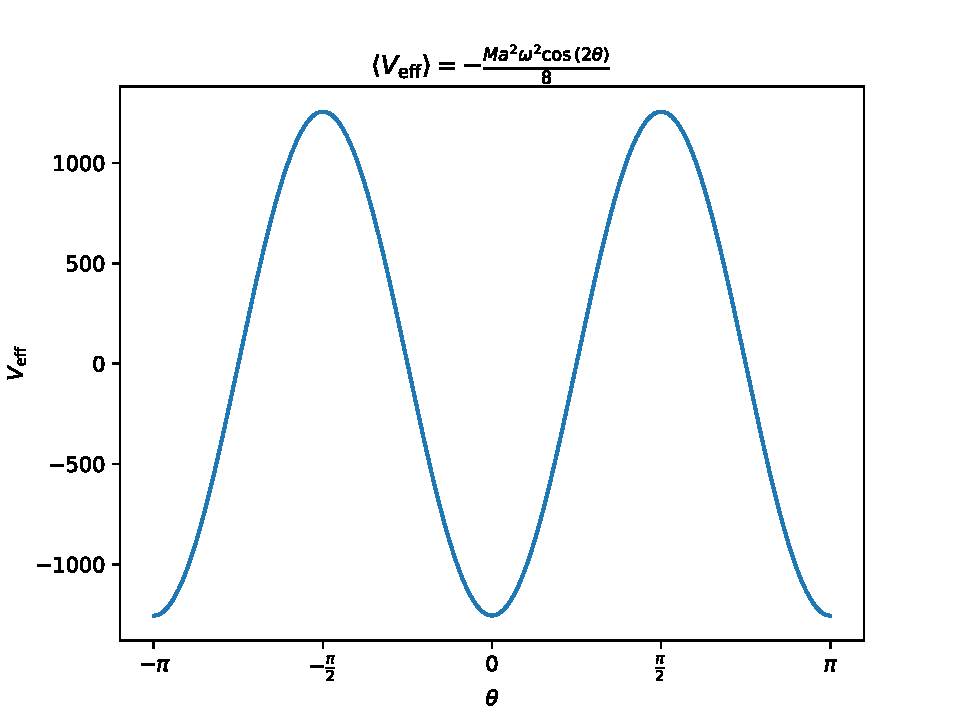
\includegraphics[width=0.5\linewidth]{Veff_without_Gravity.pdf}
    \caption{Time-averaged effective potential created by the vertically-oscillating pivot point (equation \ref{eq:averaged_potential_without_gravity}) \emph{without} gravity, using the same parameters as the numerical simulation of Figure \ref{fig:butikov_2017_figure_2} reproduced from \cite{Butikov2017KapitzaS}, namely, $l = 100$, $a = 0.2l = 20$, $g = 9.81$, $\omega = 16\sqrt{g/l}$, and $M = 1$.}
    \label{fig:ButikovKapitzaVeff_without_Gravity}
\end{figure}
From Figure \ref{fig:ButikovKapitzaVeff_without_Gravity}, it is clear that for small deviations from the inverted position, the pendulum, akin in this picture to a particle in a terrain, will roll back down to the stable inverted equilibrium point $\theta = 0$ radians.
\par Finally, to get the complete picture, including gravity appends a destabilizing $Mgl\sin(\theta)$ term to the total averaged effective torque, yielding the formula
\begin{equation}
    \left<T_{\text{in}}\right> = -\dfrac{M\omega^2 a^2}{4}\sin(2\theta) + Mgl\sin(\theta) \label{eq:total_averaged_eff_torque},
\end{equation}
which implies that the net averaged effective potential felt by the pendulum over one period of the pivot-point oscillation is:
\begin{align}
\left<V_{\mathrm{eff}}\right> &= \int \left(\dfrac{M\omega^2
a^2}{4}\sin(2\theta) - Mgl\sin(\theta)\right) \, d \theta \nonumber \\ &=
-\frac{Ma^{2}\omega^{2}\cos\left(2\theta\right)}{8} + Mgl\cos(\theta) + C, \quad \left(C
\in \mathbb{R}^1\right) \label{eq:averaged_potential_with_gravity},
\end{align}
shown in Figure \ref{fig:ButikovKapitzaVeff_with_Gravity}.
\begin{figure}
    \centering
    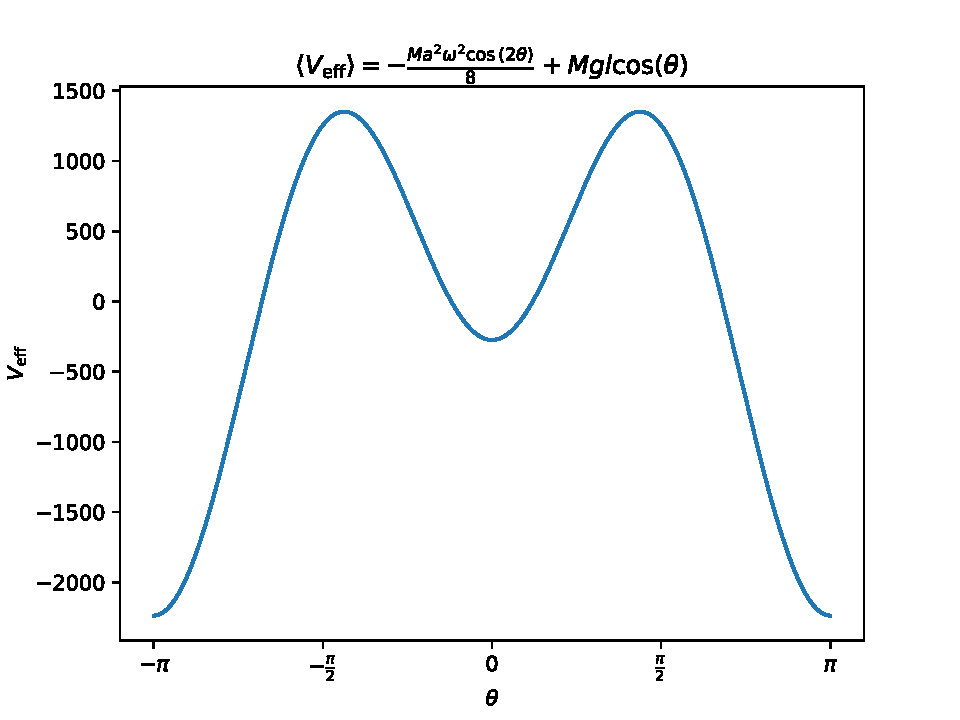
\includegraphics[width=0.5\linewidth]{Veff_with_Gravity.pdf}
    \caption{Time-averaged effective potential created by the vertically-oscillating pivot point (equation \ref{eq:averaged_potential_with_gravity}) \emph{with} gravity, using the same parameters as the numerical simulation of Figure \ref{fig:butikov_2017_figure_2} reproduced from \cite{Butikov2017KapitzaS}, namely, $l = 100$, $a = 0.2l = 20$, $g = 9.81$, $\omega = 16\sqrt{g/l}$, and $M = 1$.}
    \label{fig:ButikovKapitzaVeff_with_Gravity}
\end{figure}

Hence, for the parameter values used by Butikov in \cite{Butikov2017KapitzaS} for Figure \ref{fig:butikov_2017_figure_2}, the average effective potential near the inverted position effectively turns the originally unstable equilibrium point into a stable one. \par Another insight that one can obtain from this two-timing analysis is the maximum deviation of the slow angle $\theta$ that the pendulum may incur without falling to the $\phi=0^\circ$, non-inverted position. Butikov derives this in \cite{Butikov2017KapitzaS} by equating the averaged restoring torque generated by the pivot-point oscillation with the destabilizing torque caused by the force of gravity as follows:
\begin{align}
  \dfrac{M\omega^2
a^2}{4}\sin(2\theta) &= Mgl\sin(\theta) \nonumber \\
\Rightarrow \dfrac{a^2\omega^2}{4}\sin(2\theta) &= gl\sin(\theta)  \nonumber \\
\Rightarrow \dfrac{a^2\omega^2\left(2\sin(\theta)\cos(\theta)\right)}{4} &= gl\sin(\theta)  \nonumber \\
\Rightarrow \dfrac{a^2\omega^2\cos(\theta)}{2} &= gl\sin(\theta)  \nonumber \\
\cos\left(\theta_{\mathrm{max}}\right) &= \dfrac{2gl}{a^2\omega^2} \label{eq:max_slow_angle_dev}.
\end{align}
For the parameter values used in the simulation of Figure \ref{fig:butikov_2017_figure_2}, $\theta_{\mathrm{max}} \approx 78.74^\circ$, which agrees with the value $78.7^\circ$ that Butikov reports in \cite{Butikov2017KapitzaS}. However, this is only a restriction on $\theta$; recall that $\phi = \theta + \delta$, where $\delta \sim (z \cdot \sin(\theta)) / l$. Since, for the parameters from Figure \ref{fig:butikov_2017_figure_2}, $z = 0.2 l \sin(\omega t)$, which gives us $\delta \sim 0.2 \sin(\omega t)\sin(\theta)$. Using $\theta_{\mathrm{max}} \approx 78.74^\circ$, we get that $\sin(\theta_{\mathrm{max}}) \approx 0.981$ and thus (for the parameters from Figure \ref{fig:butikov_2017_figure_2}):
\begin{equation}
    \delta(t) \sim 0.2\cdot 0.981 \cdot  \sin(\omega t) \approx 0.196 \cdot \sin(\omega t) \approx 11.24^\circ \cdot \sin(\omega t),
\end{equation}
which then gives us an lower-bound for $\phi$ (for the parameters from Figure \ref{fig:butikov_2017_figure_2})
\footnote{The ``$180^\circ -$'' comes from the fact that Figure \ref{fig:ButikovKapitzaFig3bTopMoreDetailedGravity} is reflected about the horizontal axis relative to the convention of $\phi$ being the angle from the bottom (stable without vertical pivot-point oscillations) position that's followed in the Figure \ref{fig:butikov_2017_figure_2} simulation.}:
\begin{equation}
    \phi_{\mathrm{min}} \approx 180^\circ - \left(78.74^\circ + 11.24^\circ\right) = 90.06^\circ,
\end{equation}
which uses an over-estimation of $\delta(t)$ since $\delta$ will almost never be $\delta_{\mathrm{max}}$. Nevertheless, for this example, the destabilizing transition occurs decently close to $\phi_{\mathrm{min}}$, namely, around $\phi_0 = 91^\circ$; as seen in Figure \ref{fig:ButikovKapitza2017Figure2_phi0_92_to_91}.
\par To conclude this section, we provide, for the reader's hopeful amusement, the dynamic vector field for \ref{eq:Kapitza_pendulum_gen_framework_form} using the parameter values considered in this section, \href{https://anvaka.github.io/fieldplay/?cx=-5.4424&cy=0.2769999999999999&w=6.611800000000001&h=6.611800000000001&dt=0.005&fo=0.998&dp=0.009&cm=2&vf=vec2%20get_velocity%28vec2%20p%29%20%7B%0A%20%20vec2%20v%20%3D%20vec2%280.%2C%200.%29%3B%0A%20%20float%20g%20%3D%209.81%3B%0A%20%20float%20l%20%3D%20100.0%3B%0A%20%20float%20omega_0%20%3D%20sqrt%28g%2Fl%29%3B%0A%20%20float%20gamma%20%3D%20omega_0%20%2F%2010.0%3B%0A%20%20float%20a%20%3D%200.2*l%3B%0A%20%20float%20omega%20%3D%2016.0*sqrt%28g%2Fl%29%3B%0A%20%20float%20t%20%3D%20frame%2F100.0%3B%0A%20%20%2F%2F%20float%20t%20%3D%201.0%3B%0A%0A%20%20v.x%20%3D%20p.y%3B%0A%20%20v.y%20%3D%20-2.0*gamma*p.y%20-%20%28%28g%2Fl%29-%28a%2Fl%29*omega*omega*cos%28omega*t%29%29*sin%28p.x%29%3B%0A%20%20return%20v%3B%0A%7D&code=vec2%20get_velocity%28vec2%20p%29%20%7B%0A%20%20vec2%20v%20%3D%20vec2%280.%2C%200.%29%3B%0A%20%20float%20g%20%3D%209.81%3B%0A%20%20float%20l%20%3D%20100.0%3B%0A%20%20float%20omega_0%20%3D%20sqrt%28g%2Fl%29%3B%0A%20%20float%20gamma%20%3D%20omega_0%20%2F%2010.0%3B%0A%20%20float%20a%20%3D%200.2*l%3B%0A%20%20float%20omega%20%3D%2016.0*sqrt%28g%2Fl%29%3B%0A%20%20float%20t%20%3D%20frame%2F100.0%3B%0A%20%20%2F%2F%20float%20t%20%3D%201.0%3B%0A%0A%20%20v.x%20%3D%20p.y%3B%0A%20%20v.y%20%3D%20-2.0*gamma*p.y%20-%20%28%28g%2Fl%29-%28a%2Fl%29*omega*omega*cos%28omega*t%29%29*sin%28p.x%29%3B%0A%20%20return%20v%3B%0A%7D&pc=100000}{here}.

\begin{figure}
    \centering
    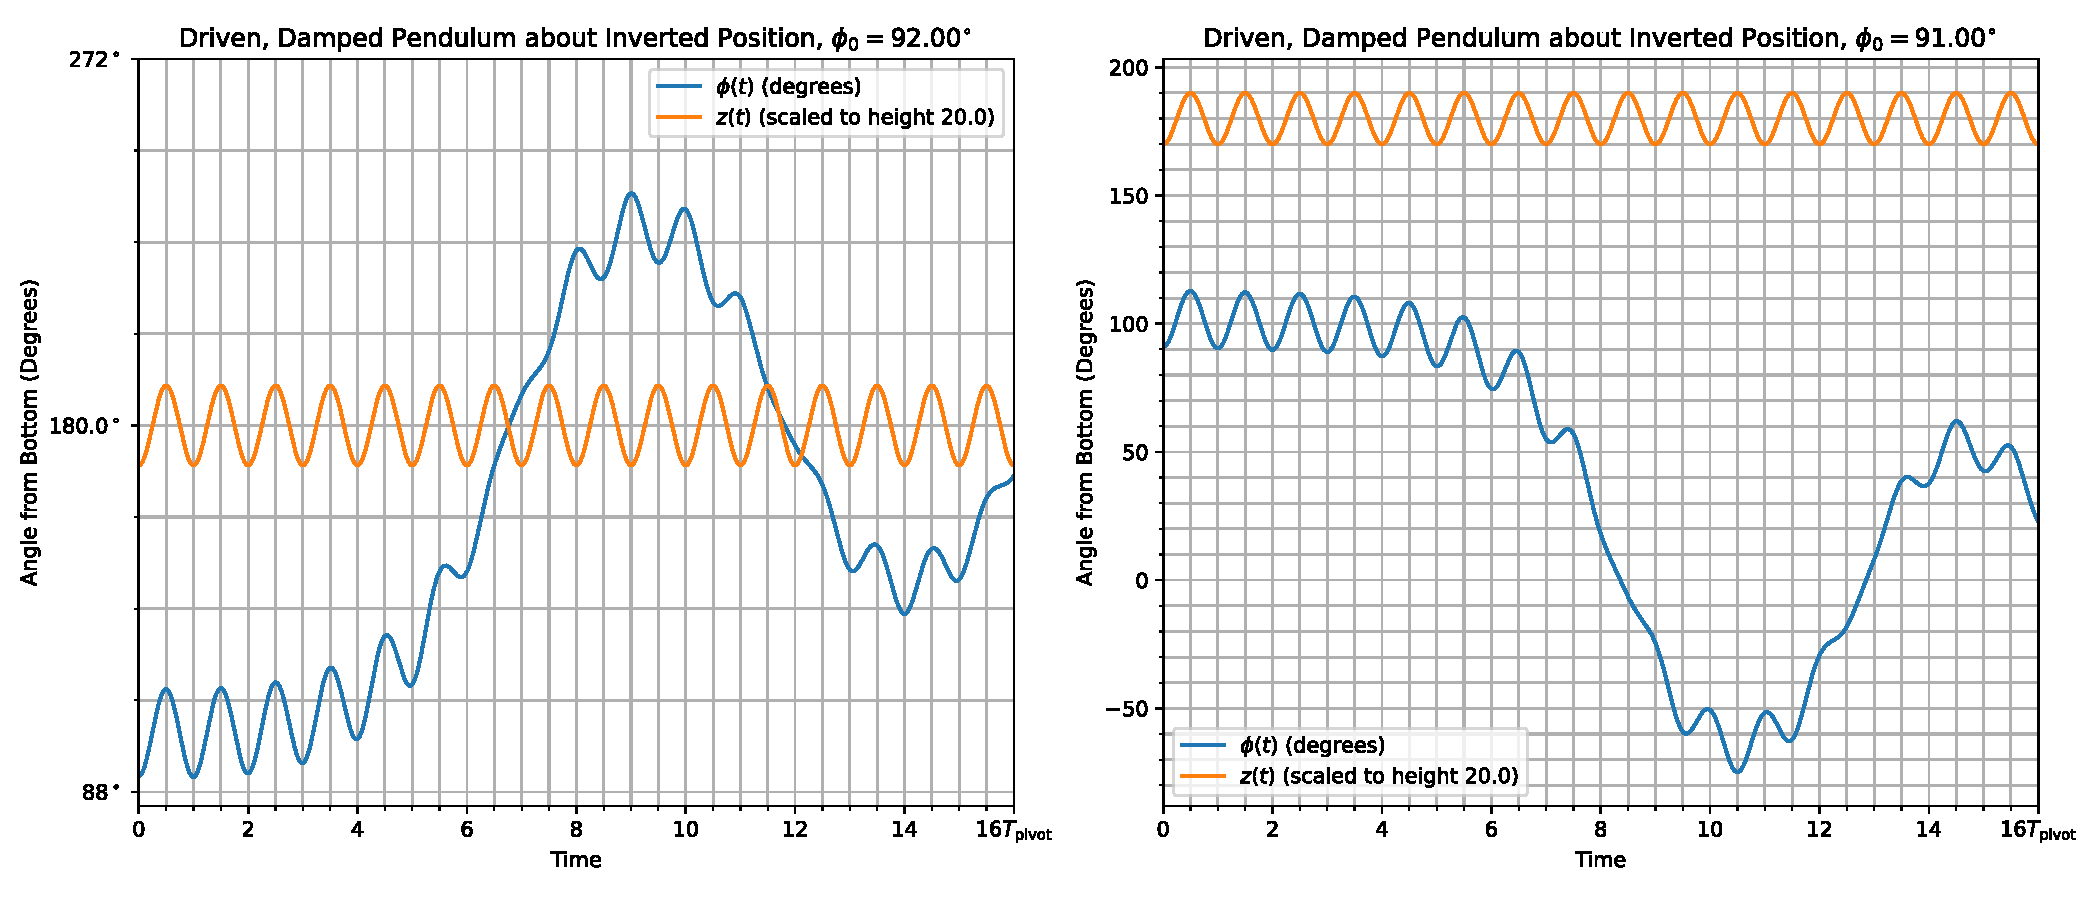
\includegraphics[width=\linewidth]{ButikovKapitza2017Figure2_phi0_92_to_91.pdf}
    \caption{Destabilizing transition that occurs from $\phi_0 = 92^\circ$ to $\phi_0 = 91^\circ$, using the same parameters as the numerical simulation of Figure \ref{fig:butikov_2017_figure_2}, namely, $l = 100$, $a = 0.2l = 20$, $g = 9.81$, and $\omega = 16\sqrt{g/l}$.}
    \label{fig:ButikovKapitza2017Figure2_phi0_92_to_91}
\end{figure}

\subsection{Linear Stability}
The time-averaging approach, while physically insightful, is only valid for a few key assumptions; namely, that the amplitude of the pivot point vibration $a$ is ``small'' compared to the length of the rod $l$, \emph{and} that the pivot-point oscillation frequency $\omega$ is ``large'' compared to the natural frequency of oscillation $\omega_0 = \sqrt{g/l}$. 
%i dont know if edward will mention the constraints or not, its not that big of deal where it goes but it should be talked about somewhere so he doesn't discuss it, then put it here as a lead in. 
\par The following approach, on the other hand, is the most standard method for analyzing stability of fixed points; it is presented in \cite{Butikov2017KapitzaS} \cite{kim1998hu} \cite{kapitsa1951jetp} and almost all literature discussing the parametrically forced pendulum. This provides more concrete insight into the parameters which stabilize the inverted position.

Our only nonlinear term is $\sin{\phi}$, so we can use a Taylor polynomial expansion about the inverted position $\phi = \pi$ to arrive at
\begin{equation}
    \ddot{\phi} - \left(\dfrac{g}{l} - \dfrac{a}{l}\omega^2 \cos(\omega t)\right)(\phi-\pi) = 0            
    \label{eq:linear_inv},
\end{equation}
Damping can be ignored for now as it has little effect on the linear stability of the inverted position. Making the transformation $\theta = \phi-\pi$ and $\tau=t\omega$ we obtain the dimensionless form of equation~\eqref{eq:linear_inv} 
\begin{equation}
    \ddot{\theta} - \left(k - m \cos(\tau)\right)\theta = 0
    \label{eq:mathieu},
\end{equation}
where $k = \frac{g}{l\omega^2}$ and $m =a/l$. Equation~\eqref{eq:mathieu} is a canonical form of the Mathieu equation. This equation is one of the simplest forms of a linear differential equation with periodic coefficients and is used to study parametric resonance problems. Floquet theory is most commonly used to analyze the stability of solutions to this system. This method examines the growth or decay of a small perturbation over one period to classify stability. 

In this framework, the regions of stability for the $\theta=0$, $\dot{\theta}=0$ solution in $(m,k)$ parameter space to this equation are mapped by the Ince-Strutt diagram shown in Figure~\ref{fig:stab_diag_mathieu}a. The blue regions are stable while the yellow regions are unstable parameters. Stable, positive k values are associated with the stability of the inverted position. The other stable regions come from a different mode of stability due to higher parametric resonances. Since k is defined as purely positive, the other regions are irrelevant to our system. 

Most analyses end here, but the same method can be applied to equation~\eqref{eq:linear_inv} if we fix two parameters and plot the parameter space for the other two. Figure~\ref{fig:stab_diag_mathieu}b is the stability diagram in amplitude and frequency of oscillation space for $l=1, g=9.81$.  

\begin{figure}[h]
    \centering
    \begin{subfigure}[b]{0.45\textwidth}
        \centering
        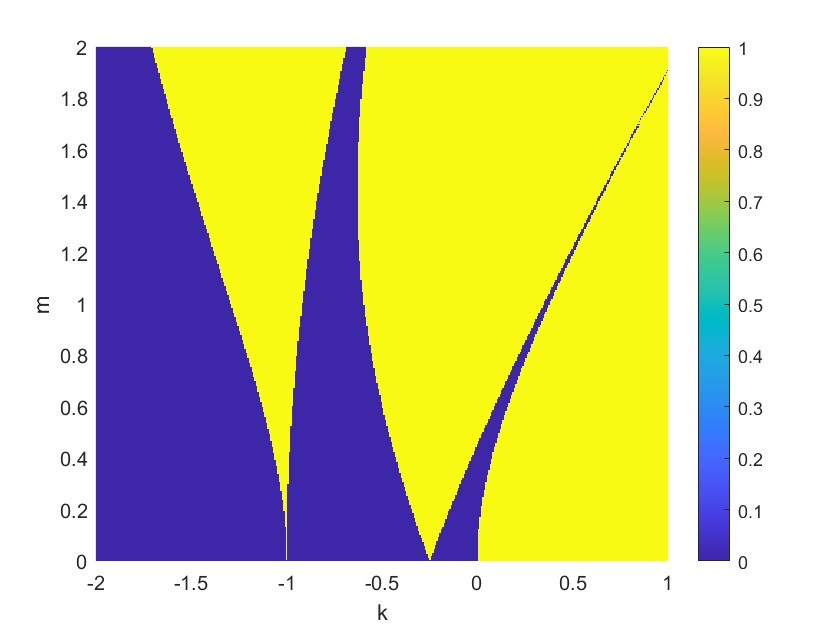
\includegraphics[width=\linewidth]{Stab_Diag_Floq_mathieu.jpg}
    \end{subfigure}
    \hfill
    \begin{subfigure}[b]{0.45\textwidth}
        \centering
        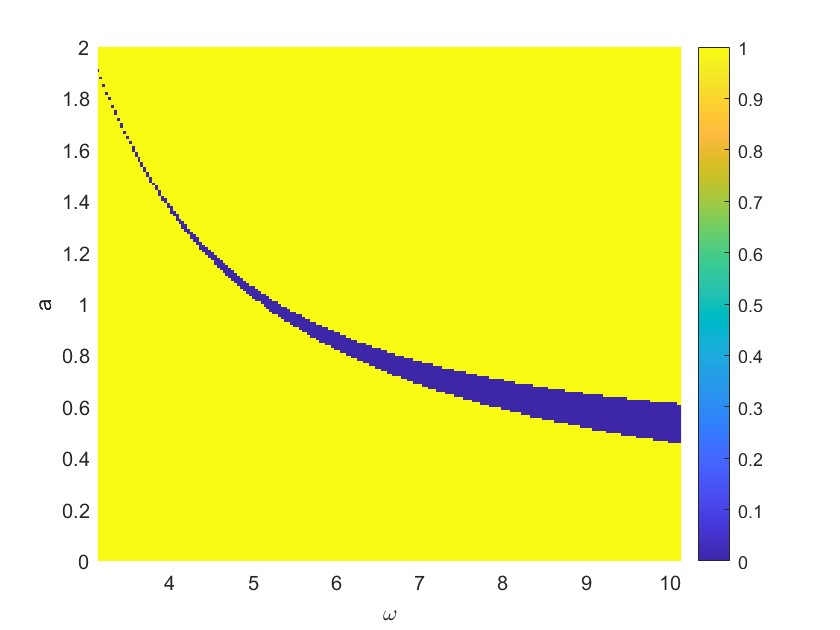
\includegraphics[width=\linewidth]{Stab_Diag_Floq_invPend.jpg}
    \end{subfigure}
    \caption{Stability diagrams for Mathieu system (equation \ref{eq:mathieu}, left), and inverted pendulum system (equation \ref{eq:linear_inv}, right). The blue regions are stable and the yellow ones are unstable.}
    \label{fig:stab_diag_mathieu}
\end{figure}

\section{Nonlinear Dynamics}\label{sec:nonlinear_dynamics}
With a foundational understanding of the stability of the inverted position, we can now analyze the dynamics of the full damped, nonlinear system. Using the same transformation for relating equation~\eqref{eq:linear_inv} to equation~\eqref{eq:mathieu}, we transform equation~\eqref{eq:Kapitza_pendulum_system} to arrive at the damped nonlinear Mathieu equation 
\begin{equation}
    \ddot{\theta} +c\sqrt{k}\dot{\theta} - \left(k - m \cos(\tau)\right)\sin(\theta) = 0
    \label{eq:damped_mathieu}
\end{equation}
where $c = \gamma\sqrt{l/g}$ and $\theta=0$ denotes the inverted position. This form for the damped Mathieu deviates from that presented in \cite{kim1998hu} to provide a closer comparison between the full system and the undamped, linear system. Nonetheless, the equation behaves the same and our results translate correctly. The most notable difference the addition of damping makes to our system is the possibility of re-stabilization of the inverted position as the amplitude is increased past the initial stable region. This recovery of stability is shown in figure \ref{fig:Damped_stability_diag}, a recreation of stability diagrams from \cite{kim1998hu} using our version of the damped Mathieu. We will now turn our attention to other solutions of this equation.
\begin{figure}[h]
    \centering
    \begin{subfigure}[b]{0.32\textwidth}
        \centering
        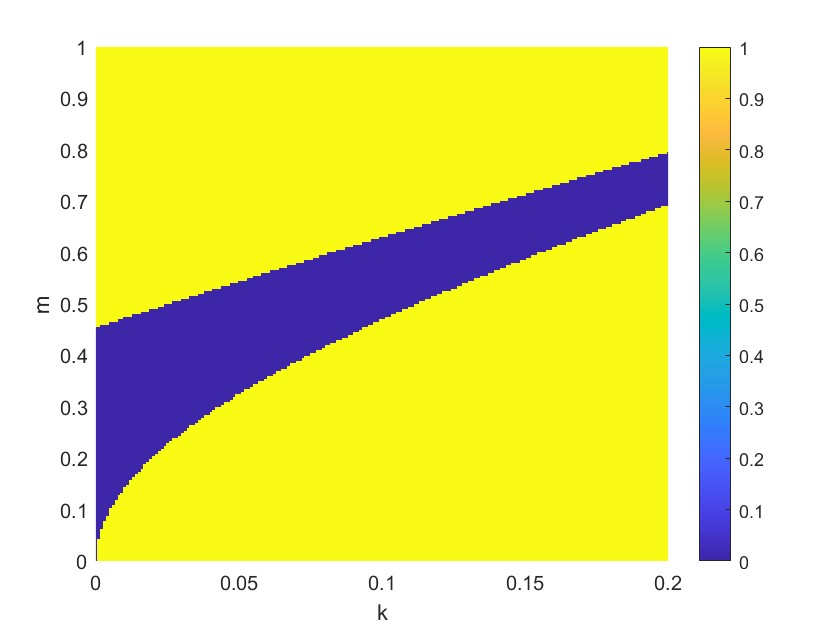
\includegraphics[width=\linewidth]{DAmp_stab_0_1.jpg}
    \end{subfigure}
    \hfill
    \begin{subfigure}[b]{0.32\textwidth}
        \centering
        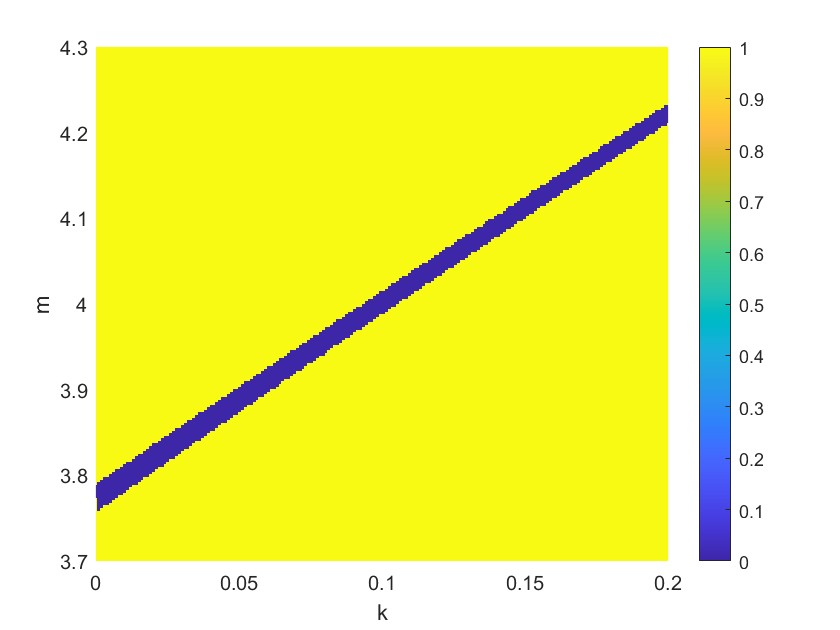
\includegraphics[width=\linewidth]{DAmp_stab_37_43.jpg}
    \end{subfigure}
    \hfill
    \begin{subfigure}[b]{0.32\textwidth}
        \centering
        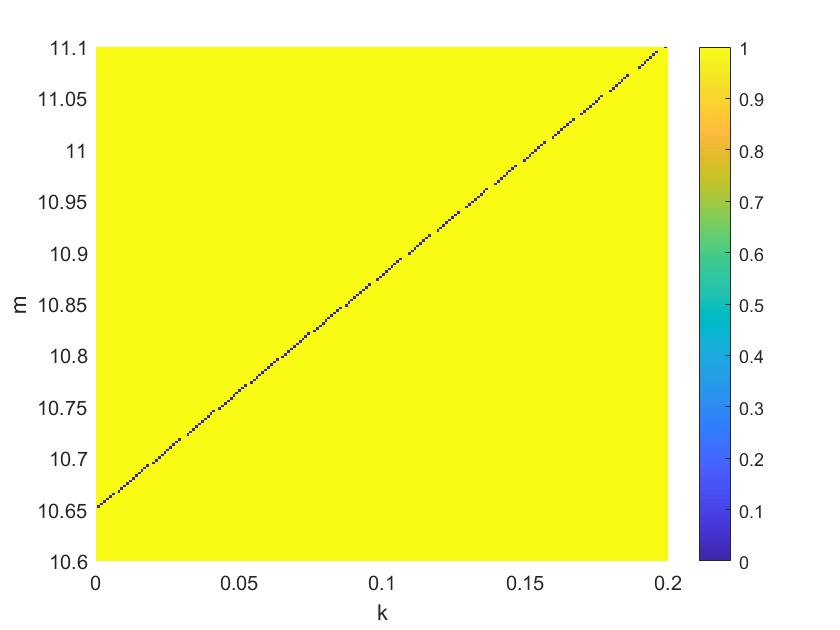
\includegraphics[width=\linewidth]{DAmp_stab_1060_1110.jpg}
    \end{subfigure}
    \caption{Three regions of stability for the same range of k values for $c=0.2$. Blue represents stable parameters. These regions exist in the undamped equation, but they are too thin for physical relevance. The more damping is increased, the larger these regions become. }
    \label{fig:Damped_stability_diag}
\end{figure}

\subsection{Limit Cycles and the Poincare Map}
In this section we review the work done in \cite{kim1998hu} to classify the stability of limit cycles in the system and prove the existence of bifurcations. When we reduce the second-order differential equation \eqref{eq:damped_mathieu} to a system of two first-order differential equations 
\begin{align}
\begin{cases}
    \dot{x} &= y \\
    \dot{y} &= -2c\sqrt{k}y+(k-m\cos(\tau))\sin(x)
\end{cases}
\label{eq:damped_system},
\end{align}
we can observe that the system has space inversion symmetry, i.e., the transformation $S:x\rightarrow-x, ~y\rightarrow-y, ~t\rightarrow t$ leaves \eqref{eq:damped_system} unchanged. With this being the case, we can more accurately classify bifurcations later on.  

To observe possible limit cycles and bifurcations, we can construct a Poincaré time-1 map. This is a discrete mapping which reduces a continuous-time, time-periodic system to a discrete-time map. Essentially, the map captures the system's state once every period (i.e., at $\tau=0,2\pi,4\pi,...$). One begins by choosing an initial state $z_0=(x_0,y_0)$ at $\tau=\tau_0$ and integrates the system from $\tau_0$ to $\tau_0+2\pi$. The resulting state $z_1$ is recorded and used as the initial condition for integration of the next period. The transformation $z_m\rightarrow z_{m+1}$ is the Poincare map denoted as $z_{m+1}=P(z_m)$.

A period-q orbit under this system will satisfy the condition $P^q(z^*)=z^*$, where $P^q$ denotes the application of the map q times. Again, the stability of these orbits can be analyzed through Floquet theory by linearizing our system about the orbit $z^*$ and using an integration period of $q \cdot 2\pi$ rather than $2\pi$. The linearized damped Mathieu system is given by 
\begin{equation}
    \left[
    \begin{matrix}
        \dot{u} \\ \dot{v}
    \end{matrix}
    \right] = 
    \left[
    \begin{matrix}
        0 && 1\\(k-m\cos(\tau))\cos(x^*) && -2c\sqrt{k}
    \end{matrix}
    \right]
    \left[
    \begin{matrix}
        u \\v
    \end{matrix}
    \right].
\end{equation}
Fortunately, we do not have to find these fixed points to analyze their stability. Through Floquet theory, it is known that the determinant of the monodromy matrix $M$ for a period $q$ is given by $\text{det}M = e^{\int_0^q \text{tr}J\, dt}$. In our system, tr$J$ does not depend on a fixed point, so the determinant can be solved directly. We arrive at the analytic result $\text{det}M = e^{-2c\sqrt{k}q}$ which we can use to analyze the Floquet multipliers. 

Complex multipliers are given by $|\lambda_{1,2}| = \sqrt{\text{det(M)}}$, which means our multipliers lie on a circle of radius $r=e^{-c\sqrt{k}q}$ in the complex plane. The range of this radius is (0,1), so the multipliers never cross the unit circle on the complex plane. This proves Hopf-bifurcations do not occur in our system. If the multipliers are real, they can take any value on the real line and therefore cross values -1 and 1. Systems exhibit period-doubling bifurcation when a stable orbit loses stability via a Floquet multiplier decreasing through -1. Pitchfork bifurcation occurs when a stable orbit loses stability via a multiplier increasing through 1. This implies that the loss of stability of the inverted position will result in one of these two bifurcation cases. 

\subsection{Bifurcation Example}
An analysis of the initial bifurcations of a few specific parameter examples is given in paper \cite{kim1998hu}. Although these examples are well analyzed and offer rich insight into the possibility of period doubling into chaos, there is a lack of visual analysis beyond the first bifurcation for the given examples. Here we look at one specific case, $k=0.01$, $c=0.2$, $0.45<m<0.58$, and dive into the bifurcation beyond the first moment. 
\begin{figure}[h]
    \centering
    \begin{subfigure}[b]{0.45\textwidth}
        \centering
        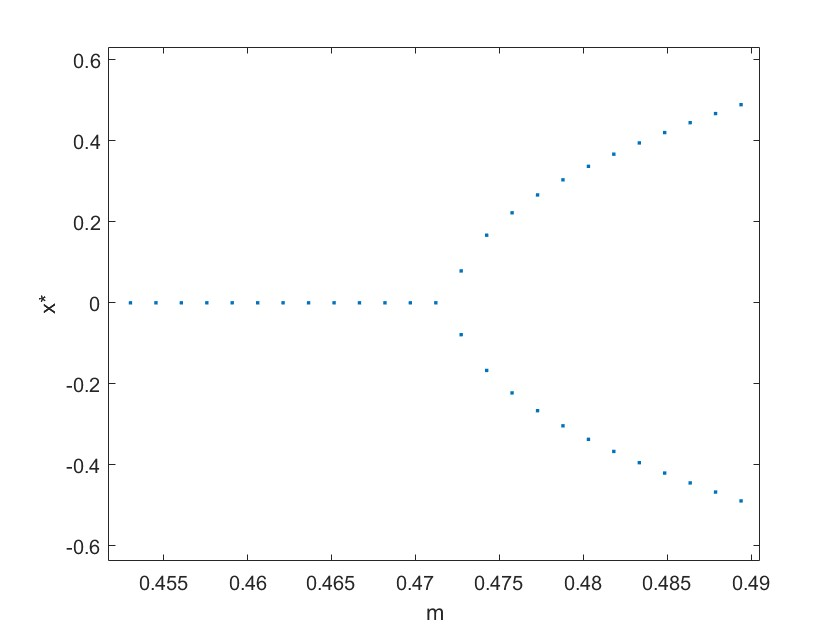
\includegraphics[width=\linewidth]{Bif_diag_poincare_2_P2.jpg}
    \end{subfigure}
    \hfill
    \begin{subfigure}[b]{0.45\textwidth}
        \centering
        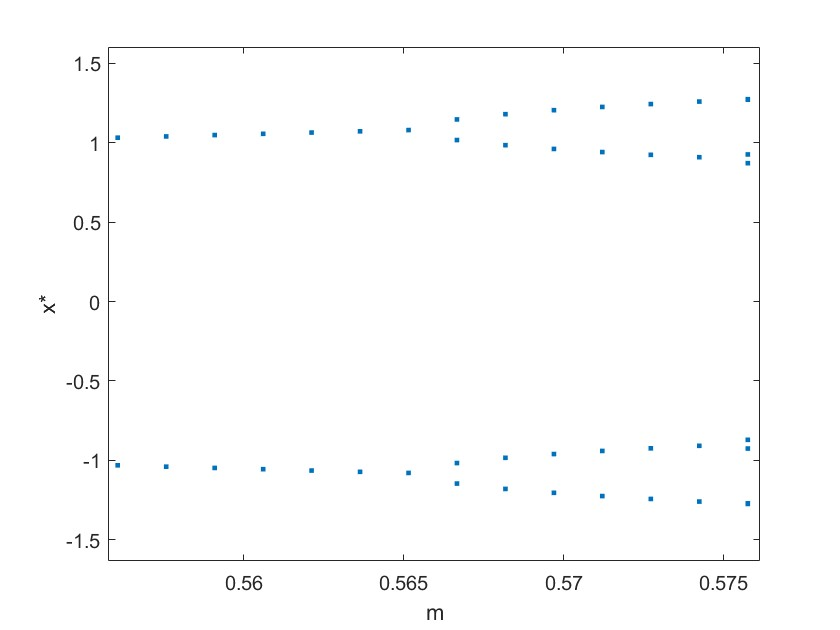
\includegraphics[width=\linewidth]{Bif_diag_poincare_2_P3.jpg}
    \end{subfigure}
    \caption{Bifurcation diagrams of the Poincaré section. These diagrams were constructed by running a thousand initial conditions through the map, discarding those not in the basin of attraction of an orbit, and plotting the final point after one hundred periods.}
    \label{fig:Bifurcation_diag}
\end{figure}

Figure \ref{fig:Bifurcation_diag} reveals three bifurcations. Since either period doubling or pitchfork bifurcation occurs, we turn to plotting phase portraits for specific values of $m$ to observe exactly what bifurcations occur.  

Figure \ref{fig:phase_port_bif} reveals the phase portraits for these specific cases of $m$. The first bifurcation after the destabilization of the inverted position is period doubling. Most would expect the next bifurcation to be another period doubling, but this is not the case. Figure \ref{fig:phase_port_bif}b consists of two different period two orbits in our system, suggesting pitchfork bifurcation. Last, one of the final states of our system that we were able to observe before what looked like chaos, was the existence of two period three orbits. It is unlikely that two period two orbits bifurcated into two period three orbits, implying that our sweep of $m$ parameter space was not fine enough to capture chaos and we actually just captured a window of periodicity within chaos for the final phase portrait. 
\begin{figure}[h]
    \centering
    \begin{subfigure}[b]{0.32\textwidth}
        \centering
        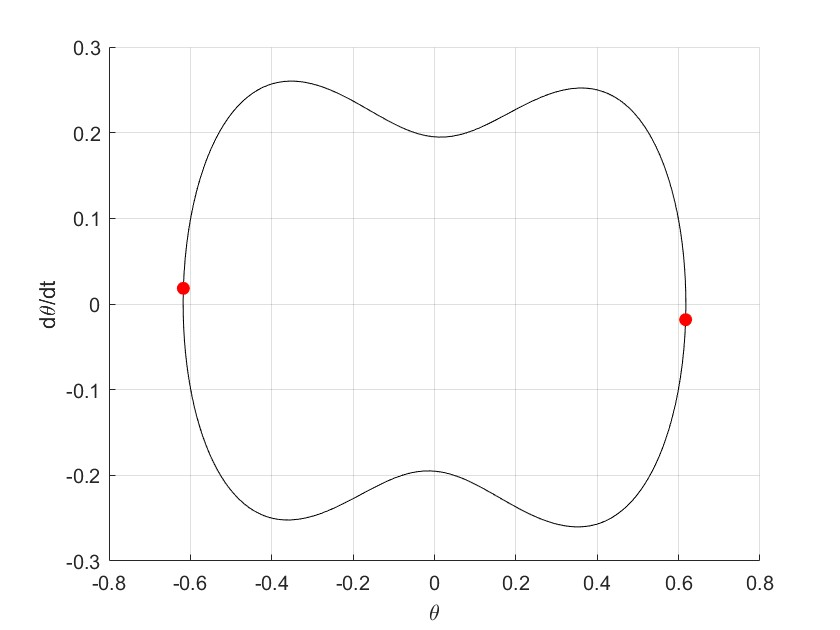
\includegraphics[width=\linewidth]{Bif_poincare_1_P2.jpg}
    \end{subfigure}
    \hfill
    \begin{subfigure}[b]{0.32\textwidth}
        \centering
        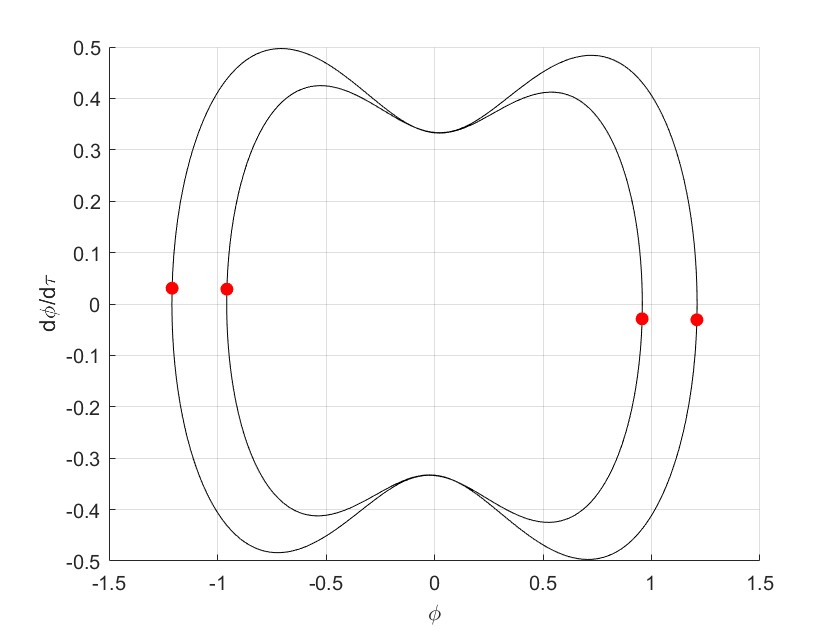
\includegraphics[width=\linewidth]{Bif_poincare_2_P2.jpg}
    \end{subfigure}
    \hfill
    \begin{subfigure}[b]{0.32\textwidth}
        \centering
        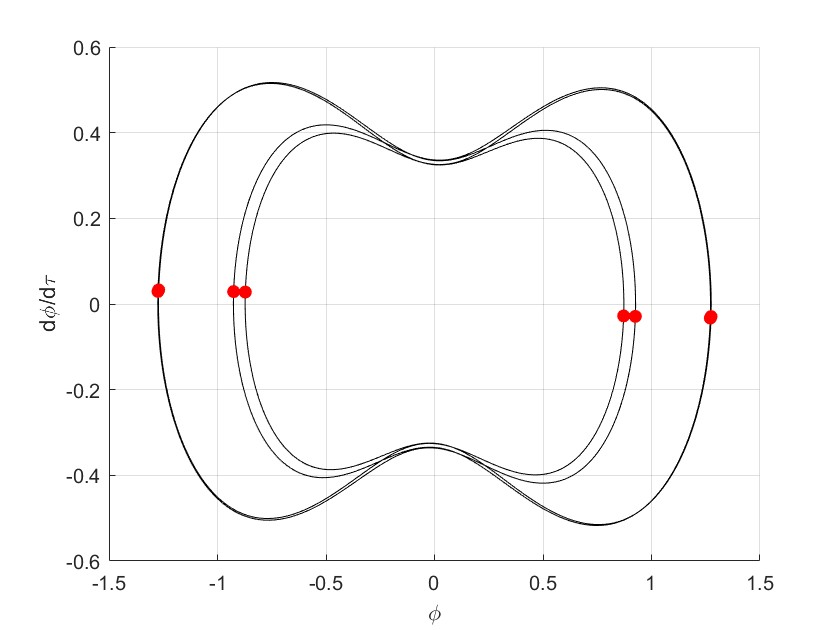
\includegraphics[width=\linewidth]{Bif_poincare_2_P3.jpg}
    \end{subfigure}
    \caption{Phase Portraits for $m = 0.4, 0.57,0.57579$ respectively of the damped nonlinear mathieu equation. (a) one period two orbit (b) two period-two orbits (c) two period-three orbits}
    \label{fig:phase_port_bif}
\end{figure}

\section{Conclusion}
The parametrically forced pendulum offers numerous opportunities to apply many forms of mathematical analysis. We carried out a detailed application of time-averaging techniques that revealed fundamental behaviors of the system. Our understanding of the occurrences of these behaviors was fine-tuned through linearization of the problem and the relation to the Mathieu equation, a widely researched system. Beyond the stabilization of the inverted position, the whole system is observed to exhibit limit cycles and bifurcation phenomena using a Poincare map and Floquet theory. Simulations of a specific case were run to validate and explore the cases of bifurcation in the system. For further explorations, a more detailed bifurcation diagram could reveal a clearer transition to chaos. Another example that should be explored is the bifurcation from the destabilization of another stability mode. 




\newpage
\bibliographystyle{plain}
\bibliography{FinalReport}
\newpage
\appendix
\section{Derivation of the Forced, Damped Pendulum Equation via Lagrangian Mechanics}\label{sec:el_derivation_butikov_eom}
We consider a pendulum of mass $m$ and length $l$ whose pivot oscillates vertically as
$$
y_0(t) = -\,a\cos(\omega t),
$$
and which is subject to viscous damping.

% ---

\subsection{Coordinates and Kinematics}

- \textbf{Pivot motion}:
  $$
    y_0(t) = -\,a\cos(\omega t)
    \quad\Longrightarrow\quad
    \ddot y_0(t) = +\,a\,\omega^2\cos(\omega t).
  $$
- \textbf{Bob position}:  
  Taking downward as positive $y$,
  $$
    y = y_0 + l\cos\phi.
  $$
- \textbf{Bob velocity}:  
  $$
    \dot y = \dot y_0 - l\,\dot\phi\,\sin\phi.
  $$
- \textbf{Kinetic energy}:  
  $$
    T = \tfrac12\,m\,\dot y^{2}
      = \tfrac12\,m\,\left(\dot y_0 - l\,\dot\phi\,\sin\phi\right)^{2}.
  $$

% ---

\subsection{Potential Energy}

- \textbf{Gravitational potential} (up to an irrelevant function of $t$):
  $$
    V = m\,g\,y = m\,g\,(y_0 - l\cos\phi)
      \sim m\,g\,l\cos\phi.
  $$

% ---

\subsection{Lagrangian}

Discarding total time–derivatives depending only on $y_0(t)$,
$$
L = T - V
  = \tfrac12\,m\,l^2\,\dot\phi^{2}
    - m\,l\,\dot y_0\,\dot\phi\,\sin\phi
    + m\,g\,l\cos\phi.
$$

% ---

\subsection{Rayleigh Dissipation Function}

Assume a damping torque proportional to $\dot\phi$:
$$
\mathcal{F} = \tfrac12\,b\,\dot\phi^{2},
\qquad
Q_\phi = -\,\frac{\partial\mathcal{F}}{\partial\dot\phi} = -\,b\,\dot\phi.
$$
Define $2\gamma = b/(m\,l^2)$.

% ---

\subsection{Euler–Lagrange Equation with Dissipation}

The equation of motion is
$$
\frac{d}{dt}\left(\frac{\partial L}{\partial\dot\phi}\right)
\;-\;\frac{\partial L}{\partial\phi}
\;=\;Q_\phi.
$$
Compute:  
   $$
     \frac{\partial L}{\partial\dot\phi}
     = m\,l^2\,\dot\phi \;-\; m\,l\,\dot y_0\,\sin\phi,
   $$
   $$
     \frac{d}{dt}\left(\frac{\partial L}{\partial\dot\phi}\right)
     = m\,l^2\,\ddot\phi
       - m\,l\,\ddot y_0\,\sin\phi
       - m\,l\,\dot y_0\,\dot\phi\,\cos\phi.
   $$
   $$
     \frac{\partial L}{\partial\phi}
     = -\,m\,l\,\dot y_0\,\dot\phi\,\cos\phi
       - m\,g\,l\sin\phi.
   $$
Subtracting and equating to $Q_\phi$ yields
$$
m\,l^2\,\ddot\phi + b\,\dot\phi + m\,g\,l\,\sin\phi
- m\,l\,\ddot y_0\,\sin\phi = 0.
$$
Insert $\ddot y_0 = a\,\omega^2\cos(\omega t)$
$$
m\,l^2\,\ddot\phi + b\,\dot\phi + m\,g\,l\,\sin\phi
- m\,l\,a\,\omega^2\cos(\omega t)\,\sin\phi = 0.
$$
Divide by $m\,l^2$
$$
\ddot\phi + \dfrac{b}{ml^2}\,\dot\phi + \,\dfrac{g}{l}\,\sin\phi
- \dfrac{a}{l}\,\omega^2\cos(\omega t)\,\sin\phi = 0.
$$
Use $2\gamma=b/(m\,l^2)$
$$
\ddot\phi + 2\gamma\,\dot\phi + \,\dfrac{g}{l}\,\sin\phi
- \dfrac{a}{l}\,\omega^2\cos(\omega t)\,\sin\phi = 0.
$$

% ---

\subsection{Final Equation}

$$
\boxed{
\ddot\phi + 2\gamma\,\dot\phi
+ \left(\frac{g}{l} - \frac{a}{l}\,\omega^2\cos(\omega t)\right)\,\sin\phi
= 0.
}
$$
\end{document}